\documentclass[11pt]{article}

\usepackage{graphicx}
\usepackage{multirow}
% make text wrap a figure
\usepackage{wrapfig}
% a package against words hyphenation. Perhaps, it works
\usepackage[none]{hyphenat}
\usepackage{eurosym}
\usepackage{textcomp}
\usepackage{amsmath}
% change the date format (avoid printing the day of week in the \today command)
\usepackage[ddmmyyyy]{datetime}
% control headers and footers
\usepackage{fancyhdr}
\usepackage[usenames, dvipsnames]{color}

% date separator
\renewcommand{\dateseparator}{.}

\definecolor{myGray}{gray}{0.15}

\usepackage{ifpdf}
\ifpdf
\usepackage[pdftex, colorlinks=true, urlcolor=myGray]{hyperref}
\else
\usepackage[hypertex]{hyperref}
\fi

%\textheight = 700pt
\textheight = 680pt
\hoffset = -25pt
\textwidth = 450pt
\voffset = -55pt

% header and footer
\pagestyle{fancy}
\fancyhead[L]{\textit{Ivan Martynov / +358 44 936 6589 /
\href{ivan.a.martynov@gmail.com}{ivan.a.martynov@gmail.com}}}
\fancyhead[R]{\textit{\thepage}}
\fancyfoot{}

\newcommand{\xfill}[2][2.5pt]{\dimen0=#2\advance\dimen0 by #1  \leaders
\hrule height \dimen0 depth -#1\hfill}
\newcommand{\sectitle}[1]{\MakeUppercase{\bf\ \xfill{0.25mm}\,#1}\,
\xfill{0.25mm}\phantom{\ }\\\smallskip}

% some solution for C# sign
\newcommand{\Csharp}{%
  {\settoheight{\dimen0}{C}C\kern-.05em \resizebox{!}{\dimen0}{\raisebox{\depth}{\#}}}}

% two solutions for C++ sign
\newcommand{\CC}{C\nolinebreak\hspace{-.05em}\raisebox{.4ex}{\tiny\bf +}\nolinebreak\hspace{-.10em}\raisebox{.4ex}{\tiny\bf +}}
%\def\CC{{C\nolinebreak[4]\hspace{-.05em}\raisebox{.4ex}{\tiny\bf ++}}}

\begin{document}

\begin{table}
	\begin{tabular}{p{200pt} p{120pt} p{150pt}}
	& & \multirow{7}{*}{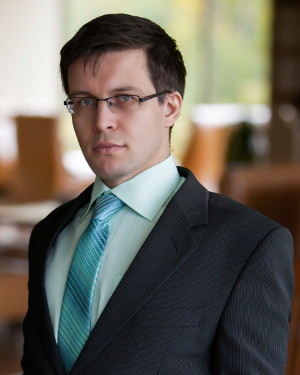
\includegraphics[width=85pt]{me_2013_09.png}}\\
	\textbf{Ivan Martynov} & \textbf{CV} &\\
	Huhtiniemenkatu 19 C 20 & \today &\\
	53810 Lappeenranta & &\\
	puh. +358 44 936 6589 & &\\
	\href{ivan.a.martynov@gmail.com}{ivan.a.martynov@gmail.com} & &\\
	Syntynyt 12.04.1982, Petroskoi & &\\
  Kansalaisuus: Suomi, Ven\"aj\"a & &
	\end{tabular}
\end{table}

%---------------------------------------------------------------------------

\noindent
\sectitle{osaaminen}
\vspace{-20pt}
\begin{itemize}
  \setlength\itemsep{1pt}
  \item Ohjelmointin kielet: C/\CC/\Csharp, Python, Java, Haskell, \textsc{Matlab}, \LaTeX,
    \textsc{HTML}
  \item Ohjelmointin konseptit: OOP, MVC, verkko (TCP/UDP), kuvank\"asittely,
    tietokonegrafiikka
  \item Tutkimus (matematiikka, ohjelmointi, kuvank\"asittely)
  \item Ajaminen (luokka B ja oma auto)
\end{itemize}

%---------------------------------------------------------------------------

\begin{flushleft}

  \sectitle{koulutus}

  \textbf{Jatkoopiskelija, Lappeenrannan teknillinen yliopisto, 2012 --}\\
  \textit{Major subject:} kuvank\"asittely, varjoen l\"oyt\"aminen\\
  \medskip

  \textbf{Diplomi-insin\"o\"ori, Lappeenrannan teknillinen yliopisto,
    2006\,--\,2008}\\
  \textit{Koulutusohjelma:} tietotekniikka; \textit{p\"a\"aaine:}
    technomathematics, \textit{sivuaine:} tietotekniikka\\
  Diplomity\"o: Computing the persistent homology of range images with alpha
    shapes\\
  \medskip

  \textbf{Diplomi-insin\"o\"ori, Petroskoin valtionyliopisto, 2002\,--\,2008}\\
  \textit{Koulutusohjelma:} matematiikka; \textit{p\"a\"aaine:} topologia,
    \textit{sivuaine:} matematiikka\\
  Diplomity\"o: About free products homeomorphisms\bigskip

  %------------------------------------------------------------------------------
  %\sectitle{muu koulutus}
  %\begin{tabular}{l l l}
  %  -- Suomen kielen kurssit, & Etel\"a-Karjalan Kansalaisopisto, &
  %    2010\,--\,2011:\\
  %  \hspace{5pt} -- Hyvin menee! 2, jatko, & 10.01.2011\,--\,13.04.2011&\\
  %  \hspace{5pt} -- Hyvin menee! 2, & 06.09.2010\,--\,13.12.2010&\\
  %  \hspace{5pt} -- Intensiivinen kurssi, & 17.05.2010\,--\,16.07.2010&\\
  %\end{tabular}

  \textbf{Coursera.org kurssit (ei todistusta):}\\
  \vspace{-10pt}
  \begin{itemize}
    \setlength\itemsep{1pt}
    \item Game Design: Art and Concepts Specialization (nelj\"a kurssia)
    \item Introduction to Interactive Programming in Python (kaksi osaa)
    \item Introduction to Game Development (Unityn perehdytys)
    \item Python for Everybody (nelj\"a kurssia)
    \item Java Programming (kaksi kurssia)
  \end{itemize}


  %------------------------------------------------------------------------------

  \sectitle{ty\"okokemus}
  \textbf{Ohjelmistokehitt\"aj\"a,Finnos Oy, 16.10.2016\,--\,14.08.2020}\\
  T\"oiss\"a olen kehitt\"anyt algoritmeja tukkien lajittelulle. Keksin ja toteutin menetelmi\"a laskemaan tukkien geometrisia ominasuuksia ja sahauskuvioita. Tein 2D ja 3D visualisointi. Olen runsaasti k\"aytt\"anyt \Csharp\ ja joskus koodanut Pythonilla ja Matlabilla.\\
\medskip
  %\textbf{Siivooja, ISS Palvelut Oy, 24.07.2014\,--\,30.5.2015}\\
  %Talojen siivoaminen (lattiat, raput, pesutupat, saunat ym.), ty\"omaan
  %  siivoamien, saunojen ja uima-allasten peseminen, lattioiden vahaus\\
  %\medskip
  \textbf{Projektip\"a\"allikk\"o, Scientific Measuring Instruments Finland Oy,
    17.09.2012\,--\,30.09.2013}\\
%  \textit{Yritys on vuonna 2011 perustettu ja on Ven\"aj\"an yrityksen (TKA)
  %  tyt\"aryhti\"o aikoa menn\"a Eurooppaan.}\\
  Olen ollut vastuullinen tehd\"a paperit\"oit\"a, j\"arjest\"a\"a kokouksia,
  hallita verkkosivuston kehittymisen ja muita teht\"avi\"a. Olen joskus ja
  onnistuneesti k\"aytt\"anyt Suomen kieli t\"oiss\"ani\\
  \medskip
  \textbf{Nuorempi tutkija, Lappeenrannan teknillinen yliopisto,
    01.05.2010\,--\,30.04.2011}\\
  %\textit{Yritys on vuonna 1969 perustettu tekniikan ja talouden yliopisto.}\\
  Suoritin tutkimus tietotekniikan osastossa, konen\"a\"on laboratoriossa.
  Tutkimuksen oli siit\"a k\"ayt\"ost\"a strukturoitujen valokuviot
  rekonstruoimaan 3D objektin muoto. T\"oiss\"ani k\"aytin Matlab-ohjelmisto ja
  C++ ohjelmointikieli Linuxin k\"aytt\"oj\"arjestelm\"ass\"a\\
  \medskip
  \textbf{Internetin luokan insin\"o\"ori, Internet-yritys ``Sampo.ru'',
    Petroskoi, 06\,--\,08/2007 sek\"a 06\,--\,08/2006 (yht. 6kk)}\\
  %\textit{Yritys on Petroskoin Internet-palveluntarjoaja.}\\
  Ty\"oskentelin asiakaspalvelussa, kassaty\"o ja toimistoty\"o. Autoin
  k\"aytt\"aji\"a Internetin luokassa, tulosta, kopiointi cd palava, skannaus,
  laminaatti ym. My\"os tein Internetin varauksen sopimuksia asiakkaille\\
  \bigskip
  %\textbf{Ty\"ontekij\"a, ``Dom-Service'', Petroskoi, 07\,--\,08/2004 sek\"a
  %07\,--\,08/2003 (yht. 4kk)}\\
  %\textit{Yritys tekee jalkak\"ayt\"av\"an laattaa ja hautakive\"a.}\\ Tekeminen
  %betonia, jalkak\"ayt\"avi\"a laattaa ja hautakive\"a, kokop\"aiv\"aty\"o\\
  %\medskip
  %\textbf{Kokki, ammattikoulun ruokala, Petroskoi, 24.09.2001\,--\,16.08.2002}\\
  %Laitin l\"ampimi\"a ruokaa ja salaattia, kokop\"aiv\"aty\"o\bigskip

  %------------------------------------------------------------------------------

  % \newpage

  \sectitle{kielitaito}

  \begin{tabular}{l l}
    \textbf{Suomi:}    & hyv\"a (Suomen kielen todistus, keskitaso)\\
    \textbf{Englanti:} & erinomainen (oppilas Lappeenrannassa ja englannin
      kielen kurssit)\\
    \textbf{Ranska:}   & perusteet (Lappeenrannan teknillinen yliopiston
      kurssit)\\
    \textbf{Ven\"aj\"a:} & \"aidinkieli
  \end{tabular}\bigskip

  %------------------------------------------------------------------------------

  \sectitle{it-taidot}

  \begin{tabular}{l l}
    \textbf{K\"aytt\"oj\"arjestelm\"at:} & Windows, Linux (erinomainen),
      Mac OS X (perusteet)\\
    \textbf{Ohjelmisto:} & Office (Microsoft ja LibreOffice)\\
                         & Grafiikka (Inkscape, Gimp, Krita, Blender)\\
                         & CFD tools (Openfoam, Ansys Icem, Fluent)
                           (perusteet)\\
      \textbf{Ohjelmointi:} & C/\CC/\Csharp, Java, Python, Haskell, \textsc{Matlab}, \LaTeX, HTML
  \end{tabular}\bigskip

  %------------------------------------------------------------------------------

  \sectitle{Muut aktiivisuutta}

  \begin{table}[h]
    \begin{tabular}{p{100pt} p{307pt}}
      \textbf{8\,--\,10.06.2009} & 16$^\text{th}$ International Summer School in
      Novel Computing, kurssit:\\
      \textbf{10\,--\,14.08.2009} & \emph{Scientific Writing} ja
      \emph{Speaker and Language Recognition}\\
      \textbf{9\,--\,13.08.2010} & 17$^\text{th}$ International Summer School in
      Novel Computing, kurssi:
      \emph{Vision for Robotic Localization and Mapping}\\
      \textbf{8\,--\,11.08.2011} & 18$^\text{th}$ International Summer School in
      Novel Computing, kurssi: \emph{Fuzzy Clustering for Image Segmentation}\\
      \textbf{30.09\,--\,4.10.2013} & Workshop on Computational and Modelling
      Problems from Industry, teht\"av\"a:
      \emph{Modelling of the electrohydraulic device}\\
      \textbf{9\,--\,13.06.2014} & The 18$^\text{th}$ European Conference on
      Mathematics for Industry\\
      \textbf{23\,--\,29.09.2015} & 13$^\text{th}$ International Conference of
      Numerical Analysis and Applied Mathematics
    \end{tabular}
  \end{table}

  %------------------------------------------------------------------------------

  %\sectitle{henkil\"okohtaiset ominaisuudet}

  \sectitle{harrastukset}
  \begin{tabular}{p{\linewidth}}
    Pid\"an fyysist\"a ja henkist\"a urheilusta, ohjelmointia,
    tietokonegrafiikkaa ja tietokone peli\"a, rakentavista peleist\"a,
    lautapeleist\"a, ruoanlaitosta, tanssimista (salsa, valssi, tango,
    breakdance). K\"ayn kuntosalissa s\"a\"ann\"ollisesti (noin kolme kertaa
    viikossa). Kielitaitoani yll\"apid\"an katsomalla englanninkielist\"a
    elokuvia ja lukemalla kirjoja. Verenluovuttaja, l\"ahtien huhtikuu 2012
  \end{tabular}\bigskip

\sectitle{suosittelijat}

\begin{tabular}{p{\linewidth}}
  \textbf{Jere Heikkinen}/ \textit{Finnos Oy} / toimitusjohtaja, jere.heikkinen [at]
  finnos.fi, +358 44 336 8652\\
  \textbf{Tuomo Kauranne} / \textit{Lappeenrannan teknillinen yliopisto,
  Matematiikan ja fysiikan laitos} / tutkijaopettaja, tuomo.kauranne [at]
  lut.fi, +358 40 530 0622\\
  \textbf{Matylda Jablonska-Sabuka} / \textit{Lappeenrannan teknillinen
  yliopisto, Matematiikan ja fysiikan laitos} / tutkijatohtori,
  matylda.jablonska-sabuka [at] lut.fi, +358 40 531 3041
\end{tabular}

\end{flushleft}

\end{document}
